\documentclass[12pt,a4paper]{report}

\usepackage[utf8]{inputenc}				% Définition du jeu de caractères
\usepackage[francais]{babel}			% Mode français

\usepackage{graphicx}					% Permet d'insérer des images
\usepackage{geometry}					% Permet de redéfinir les marges
\geometry{hmargin=2.5cm, vmargin=3cm}
\usepackage{fancyhdr}					% Personnalisation des entetes et pied de page
\usepackage{lscape}						% Permet de placer une page à la verticale (Paysage)
\usepackage{hyperref}					% Rend les titres et liens cliquables
\hypersetup{colorlinks,					% Met en noir tous les titres en noir et URL en bleu
            citecolor=black,
            filecolor=black,
            linkcolor=black,
            urlcolor=blue}


\title
{
	\vspace{-4cm}
	\begin{flushleft}
		
\includegraphics[height=2cm]{visuel/logo-upemlv.jpg}
	\end{flushleft}
	\vspace{-3cm}
	\begin{flushright}
		
\includegraphics[height=4cm]{visuel/logo-imac.png}
	\end{flushright}
	
\includegraphics[width=16cm]{visuel/logo-smashtein-garbage.jpg}
	\sc{Rapport}
}
\date{\textit{14 janvier 2010}}
\author
{
	Mathieu \sc{Taillandier} \\	
	Rony \sc{Murat}	\\	
	Jordan \sc{Valnet}	\\	
	Maxime \sc{Binetruy} \\	
	Sébastien \sc{Macher} \\	
	Alexandre \sc{Huynh}
}


\pagestyle{fancyplain}
\fancyhf{}
\renewcommand{\chaptermark}[1]{\markboth{#1}{}}
\renewcommand{\sectionmark}[1]{\markright{#1}}

\fancyhead[C]{\textsl{Rapport - Smashtein Garbage}}
\fancyfoot[R]{\textbf{\thepage}}

%% Redéfinition d'une commande pour les paragraphes
\renewcommand{\paragraph}[1]{\begin{sloppypar}#1\end{sloppypar} \vspace{0.5cm}}

\begin{document}

\maketitle

\newpage
\null

\tableofcontents

\newpage
\chapter*{1. Introduction}
\addcontentsline{toc}{chapter}{1. Introduction}
\paragraph{Le jeu vidéo connait son premier âge d’or dans les années 80 grâce à des jeux comme Pac-Man ou Space Invaders et n’a depuis cessé de se développer à tous les niveaux, si bien qu’il est aujourd’hui en passe de devenir un média à part entière, au même titre que la télévision ou le cinéma.}

\paragraph{Il était donc important pour les étudiants en multimédia que nous sommes de pouvoir envisager le fonctionnement et la réalisation d’un jeu vidéo, ce que le projet Smashstein a été l’occasion de faire puisqu’il proposait de réaliser un jeu vidéo en 2.5D (3D où les déplacements du joueur sont cantonnés à un plan) doté d’une intelligence artificielle.}

\paragraph{Dans ce but nous avons procédé en deux phases principales, avec en premier lieu la \textbf{conception théorique}, comprenant la \textbf{répartition des tâches} au sein du groupe, l’\textbf{établissement d’un rétroplanning}, la réalisation de l’\textbf{architecture logicielle} et la \textbf{mise en place des conventions} de programmation. La seconde phase concerne la \textbf{réalisation} à proprement parler, à savoir la \textbf{modélisation des décors et personnages} et la \textbf{programmation en C++ de l'ensemble des fonctionnalités du jeu}, avec toutes les \textbf{difficultés techniques} qui l'accompagnent.}

\newpage
\chapter*{2. Conception}
\addcontentsline{toc}{chapter}{2. Conception}
\setcounter{chapter}{2}
\section{Organisation de l'équipe}
\paragraph{Jusqu'à maintenant, la plupart des projets que nous avions eu à faire à l'Imac se déroulaient par binôme ou au maximum trinôme. Dans ces cas-là, la gestion du groupe s'en trouvait simplifiée car la répartition du travail était simple. Dans le cas d'une équipe de six personnes, il est nécessaire de bien connaître les aptitudes, les passions et motivations de chaque membre pour en tirer le maximum pour le bien de l'équipe (\textit{plus on aime ce que l'on fait, plus on le fait bien}). De plus, nous avons eu la chance - légèrement provoquée - que chaque membre de notre équipe provient de filières très différentes et possède des connaissances et talents très complémentaires.}

\paragraph{Un projet de programmation comme Smashstein demande en effet beaucoup de connaissances et de travail dans ce domaine, c'est pourquoi la grande majorité de l'équipe s'est attelée à cette tâche à un moment ou à un autre de l'avancement. Cependant, la programmation est à un projet comme Smashstein le ciment est à un bâtiment, il est nécessaire de créer de l'enrobage et de la matière autour pour lui donner une forme plus esthétique et agréable. C'est dans cet optique que nous avons concentré la seconde partie de l'équipe dans la réalisation des éléments graphiques tel que les modèles 3D ou les décors. Un jeu sans attrait graphique peut vite perdre de son intérêt. Le dernier membre de l'équipe s'est entièrement dédié à l'univers sonore car cette fonction est bien souvent mise en défaut alors que sans elle, un jeu peut bien vite sembler fade et triste.}

\paragraph{Ainsi, nous avons su trouver dans cette équipe toutes les compétences nécessaires au bon déroulement de ce projet afin qu'il aboutisse de la meilleure des façons malgré le peu de temps qui nous était imparti.}

\newpage
\section{\'Etablissement du planning}


\subsection{Planning prévisionnel}
\vspace{0.5cm}

\paragraph{Avant de démarrer le projet, il nous a semblé nécessaire de nous réunir afin de partager nos idées. Les phases de réflexion ne sont évidemment pas à négliger, puisque c'est le tremplin pour partir d'une m\^eme base. Nous savions par la suite ce qui devrait \^etre plus ou moins fait. Autrement dit, nous nous sommes répartis les t\^aches selon nos affinités avec tel ou tel domaine. C'est ainsi qu'un rétroplanning a été aussit\^ot mis en place. Ce planning prévisionnel permet de fixer quelques dates clés, d'avoir une vue d'ensemble des t\^aches à effectuer et d'avoir un repère dans la progression de ce projet.}
\vspace{0.5cm}
\hspace{-2cm}
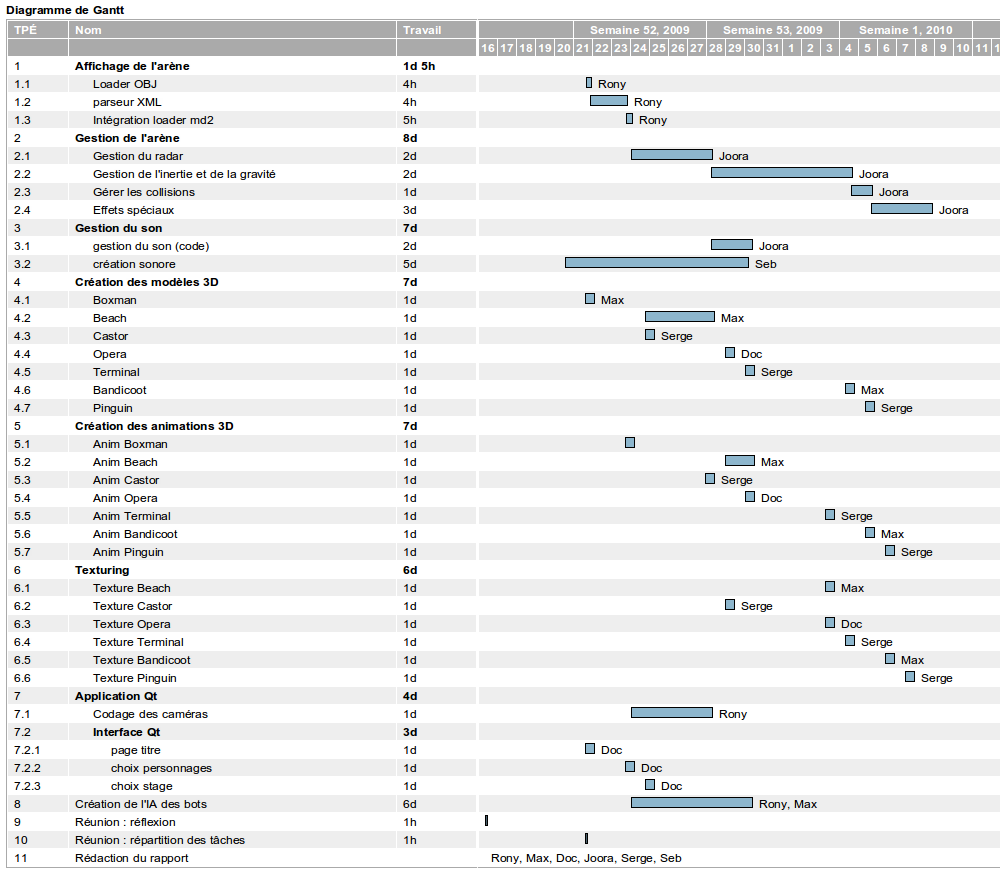
\includegraphics[scale=0.5]{visuel/retroplanning.png}
\hspace{0cm}

\subsection{Planning réel}
\vspace{1cm}

\paragraph{Après quelques semaines de travail, le planning réel a été dressé. Ce qui est intéressant, c'est de constater les changements par rapport au planning initial. Par exemple, nous avons mis en retrait la modélisation et animation de quelques personnages. Ou encore, certaines t\^aches ont pris plus de temps que prévu. Les f\^etes de fin d'année y sont probablement pour quelques choses.}

\hspace{-1cm}
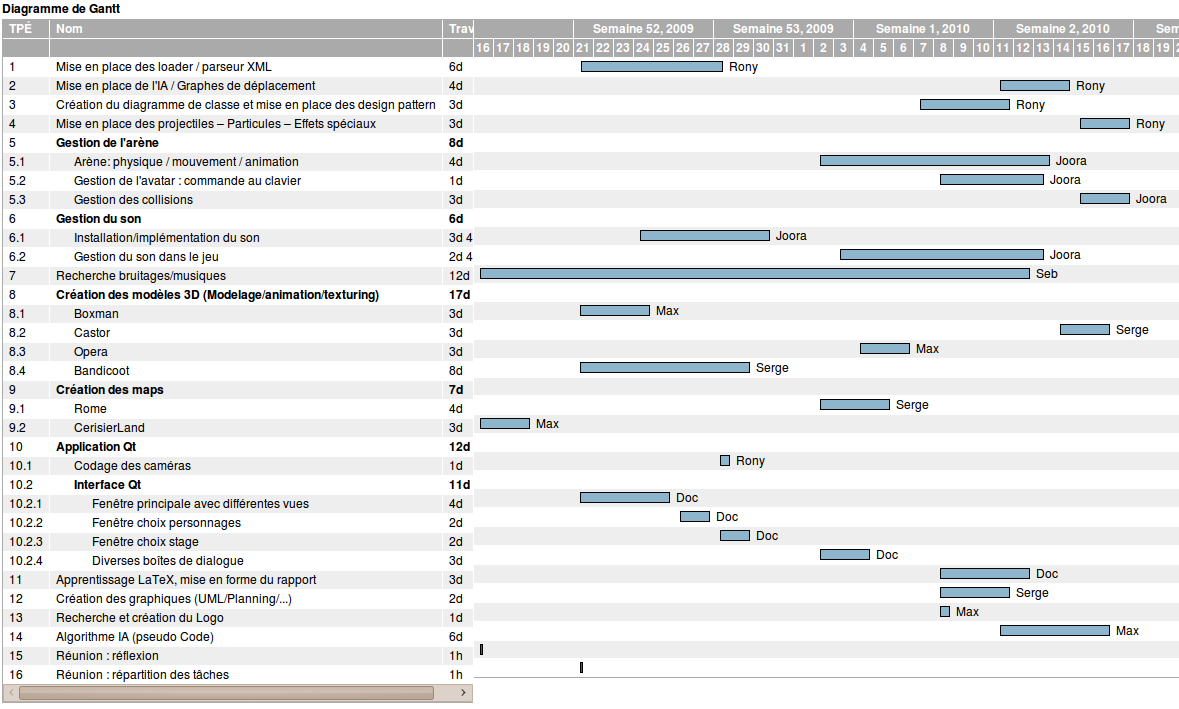
\includegraphics[scale=0.4]{visuel/planning-reel.png}
\hspace{0cm}

\newpage
\section{Organisation du travail}
\subsection{Mise en place de quelques conventions}
\vspace{0.5cm}

\paragraph{Avant de se lancer dans la programmation du jeu, nous nous sommes mis d'accord sur la façon de présenter le code. En effet, la mise en place de quelques règles d'écriture était nécessaire. Ceci permet d'avoir un code cohérent mais surtout plus compréhensible par tous les membres du groupe et donc plus facilement maintenable.}
\paragraph{Voici ces quelques règles :}

\begin{itemize}
	\item Le nom des classes, méthodes, attributs, variables, fonctions... en anglais 
	\item Le nom des classes commencent par une majuscule
	\item Les autres noms commencent par une minuscule et le mot composé qui suit par une majuscule
	\item Les accolades des blocs d'instructions sont alignées verticalement :
	\begin{verbatim}
		void method()
		{
		    ...		
		}
	\end{verbatim}
\end{itemize}


\vspace{1cm}
\subsection{Outil de travail collaboratif}
\vspace{0.5cm}

\paragraph{Deux outils de travail ont été mis en place dès le départ afin de faciliter la communication entre nous et la coordination des travaux réalisés :}

\begin{itemize}
	\item une liste de diffusion privée
	\item un système de gestion de versions
\end{itemize}

\vspace{0.5cm}

\paragraph{Tous les échanges de courriers électroniques se sont fait à travers cette adresse de diffusion : \verb?list-smashtein@pandaco.net?. \'Etant donné que nous n'étions que six dans cette liste, nous nous sommes permis de l'utiliser sans retenue. Ainsi, quelque soit la discussion, tous les membres se tenaient au courant.}

\paragraph{Concernant le choix du système de versionning, nous avons opté de mettre en place un dép\^ot centralisé de type Subversion. Nous l'avons déjà utilisé par le passé, nous étions donc plus ou moins aisés face à cet outil bien pratique. De ce fait, tous nos travaux étaient constamment synchronisés avec le dép\^ot. Afin d'éviter les conflits, nous nous mettons toujours d'accord sur quelles parties nous allons travailler.}

\newpage
\section{Architecture logicielle}
\vspace{0.5cm}
\paragraph{Dans l'optique de ce projet, nous avons décidé de réaliser un diagramme de classe qui répondrait aux principales fonctionnalités du programme de la façon la plus idéale possible. Pour ce faire, nous avons utilisé différents design patterns pour répondre à des situations bien précises. Nous n'allons bien s\^ur pas décrire la totalité de nos choix pour ce diagramme de classe dans ce rapport. Cela serait inutile et redondant. Cependant, nous expliciterons tout de même nos choix en ce qui concerne les principaux design pattern mis en place.}

\paragraph{L'arène dans ce projet est l'élément central. C'est un objet unique et nous utilisons le design pattern « \textbf{Singleton} » pour le représenter. Elle utilise une \textbf{Factory} via la classe \textit{Robots} pour générer les bots qui bénéficient d'une IA\footnote{Intelligence Artificielle} et l'avatar contrôlé par le personnage.}

\paragraph{L'arène utilise une \textit{Collection} pour stocker les objets 3D chargés via les .OBJ\footnote{Voir Section 3.6.1}. Elle gère deux collections : les objets du décor non-interactif \textit{DecorMesh} et les objets interactifs qui rentrent dans la gestion des collisions \textit{IOMesh}. Bien entendu, il existe des itérateurs pour parcourir ces différents objets dans les collections.}

\paragraph{L'arène et les bots qui possèdent une IA répondent au design pattern \textbf{Observateur}. En effet, chaque robot peut s'abonner à l'arène qui lui indique à partir de quel moment il peut effectuer une nouvelle action et lui communique les ennemis qui l'ont frappés...}

\paragraph{Une fois un bot créé, il faut être capable de lui attribuer certaines caractéristiques tel que son modèle md2, ses animations, ou encore son intelligence artificielle. Dans deux de ces cas, nous utilisons un autre design pattern pour les mettre en place. Le design pattern \textbf{Strategy} a été utilisé. L'interface \textit{Movement} en effet, permet de gérer toutes les animations du modèle 3d (run, jump, attack...) et l'interface \textit{Brain} gère, quant à elle, les « cerveaux » du bot pour pouvoir modifier dynamiquement les comportements qui vont influencer les actions du robot dirigé par l'ordinateur.}
	
\paragraph{Dans de nombreux autres cas, nous avons mis en place des interfaces qui vont faciliter la gestion des classes et des objets. Tels que tous les objets interactifs sont des obstacles. L'interface projectile pour gérer les projectiles de l'arène.}

\paragraph{Chaque \textit{Robot} implémente l'interface robot et possède des éléments tels que leur \textit{speakers} qui implémentent, eux aussi, d'autres interfaces. Nous nous sommes efforcés de mettre tout ce qui nous paraissait commun en interface afin de faciliter la gestion et la compréhension du programme.}



\newpage
\subsection{Diagramme de classe - première partie}
\vspace{0.5cm}
\hspace{-1.5cm}
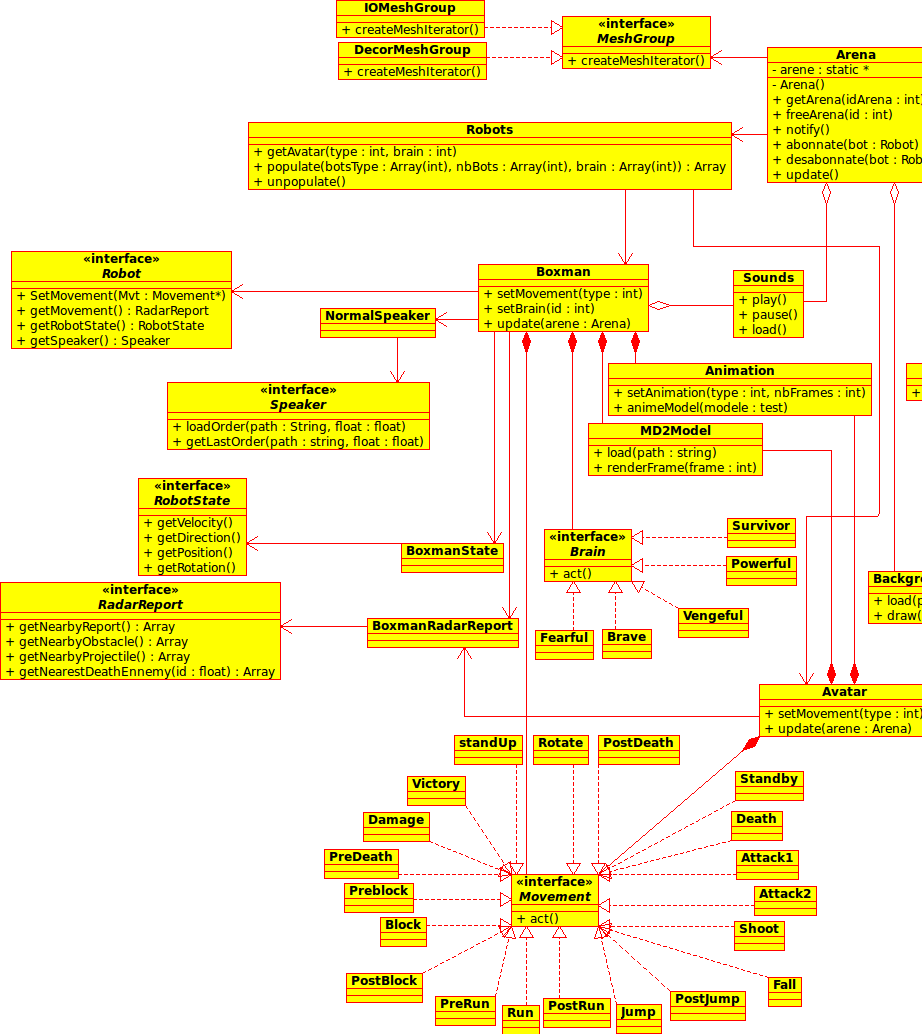
\includegraphics[scale=0.7]{visuel/uml-diagramme-classe-part1.png}

\newpage
\hspace{0cm}
\subsection{Diagramme de classe - seconde partie}
\vspace{0.5cm}
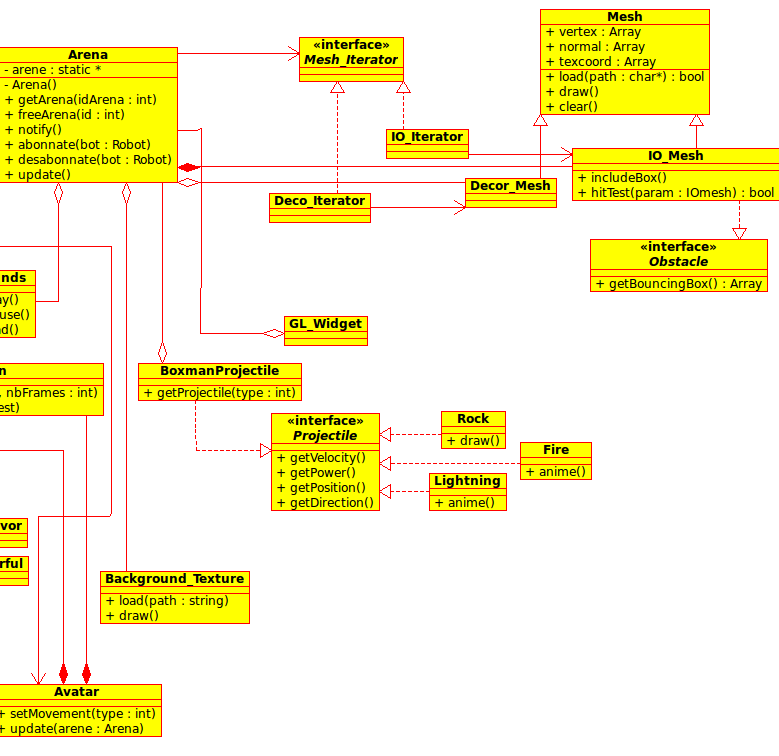
\includegraphics[scale=0.7]{visuel/uml-diagramme-classe-part2.png}


\newpage
\chapter*{3. Réalisation}
\addcontentsline{toc}{chapter}{3. Réalisation}
\setcounter{chapter}{3}
\section{Graphismes et principes d'animation}
\subsection{Thématique retenue et manifeste}

\paragraph{\'Etant conscient que le temps réservé au projet ne nous permet d'effectuer des recherches graphiques approfondies, nous avons renoncé à produire une réalisation graphique soignée et cohérente. Il serait plus juste de dire que notre recherche ne sera pas "pensée" en terme de composition, d'harmonie chromatique et de ce qui fait traditionnelement figure de règles d'or des productions graphiques ordinaires.}

\paragraph{Notre thématique retenue sera donc : GARBAGE.}

\begin{enumerate}
	\item Par GARBAGE, nous entendons le chaos le plus total, l'énergie brute de la témérité et de l'impulsivité.
	\item Les éléments essentiels de notre capharnaum seront le saugrenu, les collisions de choses paradoxales, l'aléatoire et l'absurde.
	\item Les rencontres visuelles improbables, l'hétéroclite, les associations créées seront notre poésie surréaliste.
	\item Nous ne prétendons à rien, nous ne sommes que rebuts et brouillons.
	\item Nous rejetons la logique du rationnel et privilégirons les méandres de l'esprit onirique et les liens qu'ils créent.
	\item Nous rejetons les cinq premiers points et nous ferons ce que nous pourrons libres de toute contrainte...
\end{enumerate}


\subsection{Format 3D et contraintes posées sur la modélisation}
\paragraph{Après un débat entre MD2 et MD5, nous avons opté pour le premier format plus facile à mettre en oeuvre.
En utilisant ce format-là, nous avons besoin de beaucoup plus de mémoire pour pouvoir stocker la liste de points du modèle pour chaque frame d'animation. Nous nous exposons aussi aux problèmes de normales et aux sacades inévitables des animations. Pour apporter une solution à ces problèmes, nous avons choisi de réaliser des modèles 3D en low-polygones. Nous nous sommes donc imposés \textbf{un nombre maximum de 1000 polygones pour les personnages} et de \textbf{8000 polygones pour les arènes}.}
\paragraph{Nous avons également souhaité développer dans un premier temps plusieurs personnages (de l'ordre de 5), mais nous avons réalisé que nous ne pourrions pas en modéliser et surtout animer autant. Plutôt que d'en faire beaucoup, nous avons donc décidé de nous \textbf{concentrer sur trois} d'entre eux et de \textbf{développer davantage leurs animations}.}


\subsection{Structure de l'animation}
\paragraph{Nous avons tout d'abord défini quels mouvements pourront être effectués par les personnages dans le jeu. Puis nous avons défini des priorités aux animations et dressé la liste finale que voici :}

\begin{scriptsize}\begin{verbatim}
#standby 1      // le personnage est en attente.
#prerun 2       // le personnage prend son impulsion et commence à courir.
#run 3          // -- boucle-- le personnage cours.
#jump 4         // le personnage prend une impulsion pour sauter, saute et atteint le sommet de la courbe.
#fall 5         // -- boucle-- le personnage chute après un saut.
#postjump 6     // le personnage ce réceptionne.
#attack1 7      // le personnage attaque au corps à corps selon le mode 1.
#throw 8        // le personnage attaque à distance.
#damage 9       // le personnage encaisse un coup.
#preblock 10    // le personnage se prépare à parer un coup (ou bien activer un bouclier de défense).
#block 11       // --boucle-- le personnage de protège de toute attaque.
#postblock 12   // le personnage cesse de se protéger.
#predeath 13    // le personnage encaisse un coup puissant qui l'envoi voler au loin.
#death 14       // --boucle-- le personnage en vol plané suite à un coup puissant.
#postdeath 15   // le personnage se réceptionne (tombe à terre) suite à la chute provoquée par un coup puissant.
#standup 16     // le personnage se relève pour poursuivre le combat.
#attack2 17     // le personnage attaque au corps à corps selon le mode 2.
#rotate 18      // le personnage pivote sur lui même pour changer de direction.
#postrun 19     // le personnage s'arrête brutalement après avoir courru.
#victory 20     // le personnage se manifeste au joueur de manière exubérante en cas de
                   victoire ou bien d'inactivité prolongée. 
\end{verbatim}\end{scriptsize}

\paragraph{Le terme --boucle-- indique lorqu'une animation a été prévue pour être jouée en boucle. Celle-ci s'accompagne souvent d'une "\textbf{pré-animation}" et d'une "\textbf{post-animation}". Nous avons segmenté de cette façon pour pouvoir ajuster plus finement les transitions entre animations et réduire le saut visuel provoqué par l'enchaînement d'images clés (keyframe) n'ayant rien en commun. Nous espérons ainsi limiter leur impact visuel (tenter de passer sous le seuil de perception) et augmenter la fluidité générale des mouvements des personnages.}




\subsection{Texturage}

\paragraph{Afin d'améliorer le rendu graphique des modèles en \textit{low-polygone}, nous nous somme penchés sur la réalisation de textures très détaillées. Cette solution ayant montrée ses limites (arêtes saillantes impossibles à faire disparaître...), nous avons décidé de mettre en oeuvre le "\textbf{normal mapping}".}

\paragraph{Une "\textbf{normal map}" est une textures en RVB qui définie une géométrie illusoire. Celle-ci est généralement créée à partir d'un modèle en \textit{high-polygone} qui va donner ensuite ses propriétés de réflexion de lumière au modèle \textit{low}.
Les principaux écueils de cette méthode sont :}

\begin{itemize}
\setlength{\itemsep}{20pt}
	\item la nécessité de réaliser un modèle \textit{high} (qui ne sera pas utilisé, il servira juste à la \textit{normal map}), ce qui prend beaucoup de temps.
 	\item la difficulté d'ajuster le modèle \textit{low} et \textit{high-poly} pour que la \textit{normal map} corresponde bien (risque de générer des erreurs de texturage).
\end{itemize}


\begin{figure}[h]
	\center
	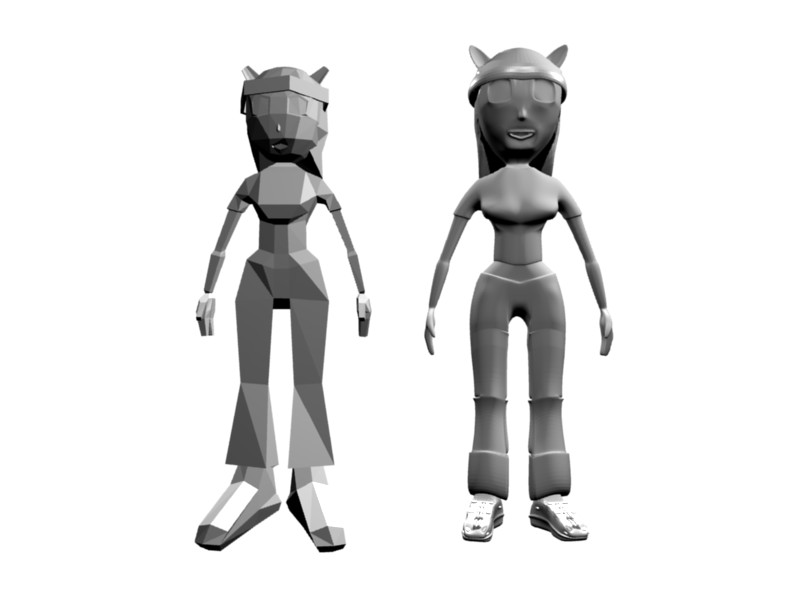
\includegraphics[scale=0.5]{visuel/low_poly_et_high_poly.jpg}
	\caption{Modèle en low-poly et high-poly}
\end{figure}


\subsection{Estimations et complexité}
\paragraph{L'essentiel des opérations coûteuses en temps de calcul se font au moment du chargement.}

\paragraph{Voici quelques-unes de nos estimations au départ du projet qui d'ailleurs ont été revues à la baisse au final :}
\begin{itemize}
	\item 1 point peut avoir au maximum 10 normales
	\item 1 triangle est composé de maximum 30 vertex
	\item 1 personnage est composé d'environ 500 triangles
	\item 1 personnage est composé d'environ 20 animations
	\item 1 animation est composé de 5 frames
	\item 1 personnage est composé de 15000 vertex
	\item 1 arène est composée de maximum 4 personnages
	\item 1 arène est composée de 140.000 triangles
	\item 5.500.000 de vertex stockés dans la carte graphique
	\item Environ 45 milions de float dans la carte graphique
\end{itemize}


\subsection{Problèmes liés au rendu graphique et solutions apportées}
\subsubsection{Implémentation des normales}

\paragraph{Le premier problème est un problème de conception concernant l'implémentation des normales : chaque vertex de nos modèles peut avoir plusieurs normales. Lorqu'il se trouve sur une arête par exemple, il appartient à deux polygones différents et possède donc deux normales mais notre implémentation des vertex n'en autorise qu'une seule.}


\paragraph{Plusieurs solutions ont été proposées : stocker un vertex par normale quitte à répéter plusieurs fois le même point : position et coordonnées de texture. Cette solution présente l'avantage d'être compatible avec la structure des Vertex Buffer Object (VBO) mais implique également un nombre de vertex stockés multiplié par quatre (estimation en moyenne), et une difficulté d'implémetnation accrue au moment de leur construction dans le loader.}



\newpage
\section{Les loaders}
\subsection{Loader OBJ}
\vspace{0.5cm}

\paragraph{Dès le départ, nous voulions avoir un rendu visuel convenable. Il nous a paru alors nécessaire de créer des arènes à partir de modèles objets en 3D modélisés et texturés via un logiciel adapté (Blender, 3DSMax). Notre choix s'est porté sur le format OBJ qui est un format simple et facile à implémenter permettant de charger facilement des objets en 3D avec des textures. En effet, chaque OBJ peut etre associé avec un MTL. Ce dernier fournit des informations sur les textures utilisées et les couleurs ambiantes et diffuses de chaque modèle. Les textures sont chargées à partir d'images PPM.}

\paragraph{La version actuelle de notre loader ne gère pas de multi-texturing sur un seul OBJ mais nous espérons avoir le temps d'implémenter la version gérant ce multi-texturing pour le rendu final.}

\paragraph{Les OBJ sont chargés dans les classes Mesh qui possèdent 2 sous-classes. En effet, afin de gérer les collisions, les Mesh sont séparés en 2 types. Les éléments de décor stockés dans les classes DecorMesh et les éléments interactifs qui sont ceux avec lesquels le joueur et les bots, pourront rentrer en collision stockés dans les classes IOMesh. Chaque IOMesh possède donc des Enveloppes pour détecter les collisions.}


Le chargement des Mesh se fait via un fichier XML qui donne les OBJ à charger. Le formatage du fichier est le suivant : Toutes les informations sur un niveau sont contenues dans une balise \verb?<map>?. Dans cette balise se trouvent quatre types de balises :


%% Création d'un type de liste pour les balises
\newenvironment{malistebalise}%
{ \begin{list}%
	{$\bullet$}%
	{ \setlength{\itemsep}{30pt}}}%
{ \end{list} }
%% Fin

\begin{malistebalise}

	\item
	{
		la balise \verb?<graph>? correpond au fichier décrivant le graphe de déplacement à utiliser pour que l'IA\footnote{Intelligence Artificielle} puisse se déplacer.
		\begin{description}
			\item[path] : chemin vers le fichier.
		\end{description}
	}
	
	\item
	{
		la balise \verb#<background># correspond à la texture de fond du niveau. Elle a comme attributs :
		\begin{description}
			\item[path] : chemin vers la texture de fond du niveau. 
			\item[width, height] : respectivement les largeurs et hauteurs de cette texture. 
			\item[x, y, z] : respectivement les positions en x, y et z du centre de la texture.
		\end{description}
	}
	
	\item
	{
		les balises \verb#<element># renseignent les OBJ des éléments à charger dans les classe DecorMesh. Elle possède comme attributs :
		\begin{description}
			\item[path] : chemin vers le fichier en .obj. 
			\item[x, y, z] : positions en x, y et z du modèle. 
			\item[xrot, yrot, zrot] : angles de rotation en degrés de l'élément respectivement sur les axes x, y et z.
		\end{description}
	}
	
	\item
	{
		les balises \verb#<mesh># renseignent les OBJ des éléments à charger dans les classes IOMesh. Elle possède les mêmes attributs que la classe élément mais donne en plus : 
		\begin{description}
			\item[xBox, yBox, widthBox, heightBox] : respectivement la position en x, y et la largeur et la hauteur de la bo\^ite qui englobe cet objet utile pour la détection des collisions.
		\end{description}
	}
	
\end{malistebalise}

\vspace{1cm}

Exemple :

\begin{scriptsize}\begin{verbatim}
<map>
   <graph path="obj/graph.txt" />
   <background path="obj/textures/clouds.ppm" width="100" height="50" x="-50" y="-15" z="-10.0"> </background>
   <mesh path="obj/map_Rome_allege.obj" x="0" y="-0.2" z="0" xrot="0" yrot="0" zrot="0" >MAP_ROME_ALLEGEE</mesh>
</map>
\end{verbatim}\end{scriptsize}



\vspace{1cm}
\subsection{Loader MD2}
\vspace{0.5cm}


\paragraph{Toutes les informations sur un bot sont données dans la balise \verb?<bot>? Dans cette balise se trouve plusieurs types de balises :}
\begin{itemize}
	\item[\verb?<name>?] : nom du modèle de bot.
	\item[\verb?<brain>?] : nom du plugin d'IA à utiliser.
	\item[\verb?<body>?] : informations sur le bot et sur le modèle MD2 à choisir. Cette balise possède comme attributs :
 	\begin{itemize}
 		\item 'velocity' : vitesse du bot.
		\item 'resistance': résistance de ce dernier.
	\end{itemize}
\end{itemize}

\vspace{1cm}

\paragraph{Elle contient également d'autres balises spécifiques au modèle MD2 :}
\begin{itemize}
	\item[\verb?<model>?] : nom du binaire MD2 à utiliser. Ses attributs :
	\begin{itemize}
		\item 'x', 'y', et 'z':  respectivement les positions x, y et z du modèle par rapport à l'origine du dessin.
		\item 'xrot', 'yrot' et 'zrot' : respectivement les angles de rotation en degré par rapport à l'origine du dessin.
		\item 'scale' : changement d'échelle à effectuer sur les 3 axes pour dessiner le modèle convenablement.
	\end{itemize}
	\item[\verb?<texture>?] : chemin vers la texture à utiliser pour afficher le modèle.
	\item[\verb?<anime>?] : chemin vers le fichier d'animation qui donne les différentes animations du modèle.
\end{itemize}

\vspace{1cm}

Exemple :
\begin{scriptsize}\begin{verbatim}
<bot>
  <name>boxman</name>
  <brain>libAINormal.so</brain>
  <body velocity="1.0" resistance="1.0">
    <model x="0.0" y="-0.2" z="0.0" xrot="0" yrot="-90" zrot="90" scale="0.013">p_boxman.md2</model>
    <texture>p_boxman.ppm</texture>
    <anime>p_boxman_anim.txt</anime>
  </body>
</bot>
\end{verbatim}\end{scriptsize}

\vspace{1cm}
	
\paragraph{Les lignes de commentaires commencent par '\#'. Dans le fichier\footnote{Voir exemple dans l'annexe} sont donnés dans l'ordre les animations :}


\begin{verbatim}
<type_animation> <frame_début> <frame_fin> <fps>
\end{verbatim}


Exemple :
\begin{scriptsize}\begin{verbatim}
#MD2 Anim p_bandicoot 
#Total : 550 frames 
#Decoupe moyenne : 5 frames per key 
#Estimation pour md2 : 70 * 2 

#standby 1 
#prerun 2 
#run 3 
#jump 4 
#fall 5 
#postjump 6 
#attack1 7 
#throw 8 
#damage 9 
#preblock 10 
#block 11 
#postblock 12 
#predeath 13 
#death 14 
#postdeath 15 
#standup 16 
#attack2 17 
#rotate 18 
#postrun 19 
#victory 20 // Indication : faire une pause à : 525 ; 530 ; 535 ; boucler de 540 à 550 

1 1 40 35
2 40 50 40
3 50 70 40
4 80 105 40
5 105 120 40
6 120 160 50
7 160 200 40
8 200 230 40
9 230 260 40
10 260 270 40
11 270 280 40
12 280 290 40
13 290 310 40
14 310 325 40
15 325 365 40
16 365 435 40
17 435 465 40
18 465 480 40
19 485 520 50
20 520 550 45
\end{verbatim}\end{scriptsize}





\vspace{1cm}
\subsection{Problèmes rencontrés}
\vspace{0.5cm}

\paragraph{Le problème que nous avons rencontrés et que nous n'avons pas compris tout de suite, vient du type de fichier utilisé pour les textures. En effet le format PPM donne une image miroir de l'image réelle. Or appliquer la texture sur le modèle MD2 requiert une image miroir alors que les OBJ utilisent l'image réelle. Étant donné que les textures des deux modèles étaient chargées en mode miroir, les textures ne s'appliquaient pas correctement. Il a donc fallu changer le mode de chargement selon le modèle sur lequel il fallait l'appliquer.}

\paragraph{Par rapport au chargement des textures, il nous était impossible de charger une et une seule fois les textures pour toutes les vues (modes porsuite, global, debug "sphérique" et libre). Chaque vue étant contenue dans un widget, il a fallu donc charger quatre fois ces m\^emes textures. Ce mode de chargement nous a semblé bien plus qu'aberrant. De plus, la consommation mémoire s'en voit alourdie, ce qui bien embêtant.}



\newpage
\section{Physiques de l'arène}
\paragraph{L'arène possède certaines lois physiques auxquelles on soumet chaque robot ou avatar.\\
Le modèle physique qui a été mis en place est le suivant :}

\paragraph{Un robot possède (via la classe \textbf{BoxmanState}) :}
\begin{itemize}
	\item une direction (vecteur3f)
	\item une accélération (vecteur3f)
	\item une vitesse (vecteur3f)
	\item une position (vecteur3f)
	\item une vitesse maximale en x, y et z (stockée dans un vecteur3f)
\end{itemize}

\vspace{0.5cm}

\paragraph{L'arène, quant à elle, possède :}
\begin{itemize}
	\item une force de gravité (vecteur3f négatif en y)
	\item une vitesse maximale pour la chute (double)
\end{itemize}

\paragraph{La physique est appliquée à chaque frame, avec une intensité proportionnelle au temps écoulé depuis la dernière frame afin d'être visuellement constante malgré des variations de fps.}

\paragraph{Elle se comporte globalement d'une façon réaliste un peu modifiée :}
\begin{verbatim}
accélération += direction
vitesse      += accélération + gravité
vitesse      /= force de frottement
vitesse      =  max(vitesse, vitesse max)
position     += vitesse
\end{verbatim}
\paragraph{L'accélération et la direction sont remises à zéro.}

\paragraph{La direction correspond à une impulsion dans un certain sens, provoquée par un ordre de l'IA/avatar. L'avantage de fonctionner ainsi permet d'avoir un démarrage progressif. Cependant trois vecteurs auraient suffi pour le même modèle.}

\paragraph{Cas particuliers : \\
 Sur le sol, on ne tombe plus. La force de gravité annulée. La force de frottement est élevée sur le sol, et quasi nulle en l'air. Cependant des mouvements ajoutent leurs propres lois et comportements en plus du modèle général. Par exemple un saut possède des lois physiques internes non réalistes pour permettre de diriger (et le plus aisément possible) le personnage en vol.}
 
 
 
\section{Mouvements}
\paragraph{Les mouvements des robots et avatars sont nombreux et plus ou moins complexes. Pour simplifier la gestion des mouvements nous avons utilisé le design pattern \textit{État} : chaque mouvement est défini dans une classe à part qui hérite de l'interface Movement, qui implémente une méthode \verb?act()?.}
\paragraph{Un robot possède un seul mouvement (en pointeur) qui peut changer via la méthode \verb?setMovement(Movement*)?.}
\paragraph{A chaque frame, la méthode \verb?act()? du mouvement du robot est appelée. Le changement de mouvement se fait par le mouvement lui-même, dans la méthode \verb?act()?.}

\paragraph{Illustrons par un exemple :}
\paragraph{Le robot a tout d'abord un mouvement "\textit{StandBy}", c'est ce mouvement-là qui est effectué. Quand le robot donne l'ordre d'avancer dans une direction, le mouvement \textit{StandBy} l'interprète et change le pointeur mouvement du robot en un nouveau mouvement "Run". La frame suivante, ce sera le mouvement \textit{Run} qui sera joué.}

\paragraph{Remarque sur le design pattern choisi :\\
Il est très approprié à la situation et a bien simplifié la gestion complexe des mouvements. Cependant, il n'évite pas certaines redondances de code lorsqu'on doit gérer les mêmes cas depuis plusieurs mouvements différents.}


\paragraph{Rôle - chaque mouvement peut ou doit :}
\begin{itemize}
	\item gérer l'animation 3D du robot,
	\item interpréter les ordres reçus par les robots,
	\item gérer les déplacements des robots
	\item changer le prochain mouvement
\end{itemize}



\section{Collisions}
\paragraph{Si rien ne se touche, il n'y a pas de jeu... Les personnages ne doivent pas traverser le décor et pouvoir se toucher entre eux. C'est le but du jeu !}
\paragraph{Nous avons donc ajouté des \textbf{boites englobantes}\footnote{Voir figure ci-dessous} autour des objets principaux : le sol, les plateformes, certains obstacles et bien sûr les robots/joueurs.}

\paragraph{Comme tout se joue sur un seul plan, il n'y a que quatre côtés à tester par objet.\\
Un test est effectué pour chaque robot sur tous les objets du décor, indiquant le cas échéant quelle face est touchée. Par exemple, si c'est la face du dessous, alors le robot est  "sur le sol" et ne tombe plus !
De même, les robots peuvent se "traverser" mais des tests sont effectués lors des coups : ai-je heurté quelqu'un ? De quel côté ? Ensuite sont gérées les conséquences (vol plané, dommages...).\\
Il en sera de même pour les projectiles lorsque nous les implémenterons.}

\begin{figure}[h!]
	\center
	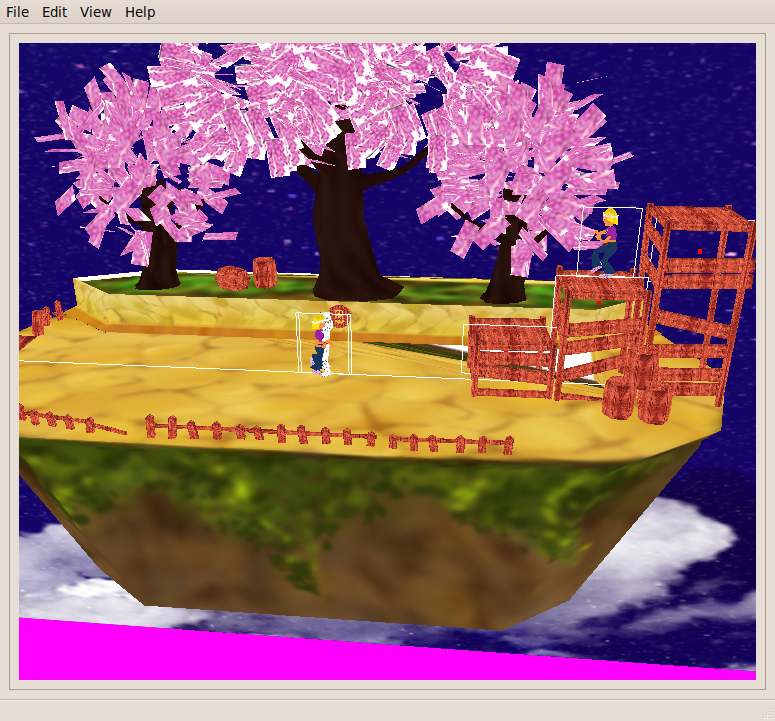
\includegraphics[scale=0.4]{visuel/capture-rev192-collision.png}
	\caption{Les bo\^ites englobantes visibles en blanc sur cette image permettent de gérer les collisions.}
\end{figure}



\newpage
\section{Les projectiles}
\vspace{0.5cm}

\paragraph{A l'heure où nous écrivons ces lignes, nous n'avons pas encore commencé la gestion des projectiles. Mais nous pouvons donner une description des fonctionnalités à implémenter.}

\paragraph{Les projectiles seront modélisés via des double billboards et des particules dans un premier temps et par des OBJ également, si nous en avons le temps. C'est la classe Arene qui gère les projectiles qui sont instanciés via la \textit{factory} \textit{BoxmanProjectile}. Le lancement d'un projectile s'effectue par la création d'un billoard et/ou d'un système de particules. Une \textit{factory} sera utilisée pour générer des modèles de particules et billboards qui seront prédéfinis dans la classe afin d'éviter d'avoir à fournir les paramètres des systèmes de particules par exemple.}

\paragraph{Un projectile est créé à chaque fois qu'un bot ou que l'avatar souhaite en utiliser et chaque type de bot possède un type de projectile qui lui est associé. Le paramétrage des particules et des billboards de chaque bot sera fait en dur dans la \textit{factory} et pourra, si nous avons le temps, être défini via le fichier XML définissant un bot.}

\paragraph{Selon le type de projectile la physique pourra ou pas être appliquée. Des projectiles très rapides ne subiront pas la physique alors que d'autres plus lent y seront soumis.}

\paragraph{Les système de particules seront également utilisés pour donner de la crédibilité au jeu. Lors de l'arrêt d'un personnage, on peut jouer de la fumée pour montrer la glissade ou faire une petite explosion quand un projectile heurte un bot ou lorsqu'un bot donne un coup.}


\newpage
\section{Intelligence artificielle}
\subsection{Fonctionnement}
\paragraph{NB : La mémoire se base sur la récupération d'un argument de "main" pour le profil du joueur et la construction d'arbres de probabilités personalisés et stockés dans des fichiers textes.}

\paragraph{L'IA est appelée lorsqu'elle reçoit le radar. Nous avons réfléchi aux actions qu'elle devait obligatoirement exécuter lors de son processus de prise de décision. De fait, nous devions avoir fixer un gameplay pour pouvoir imaginer le comportement de l'intelligence artificielle. Voici une liste des actions qui ont finalement été retenues :}

\begin{itemize}
	\item Direction droite
	\item Direction gauche
	\item Sauter
	\item Coup1
	\item Coup2
	\item Projectile
	\item Bloquer
\end{itemize}

\vspace{1cm}

\paragraph{\`A partir de ces éléments, l'IA peut : se déplacer pour s'approcher du joueur ou au contraire le fuir, atteindre des plateformes en sautant, choisir d'attaquer au corps à corps ou bien à distance. Elle peut également décider de se défendre et parer certains coups.}

\paragraph{\textbf{Mais comment l'IA allait-elle décider de l'action à effectuer ?}}

\paragraph{Après réflexion, nous nous sommes rendu compte que personne ne réagirait de manière identique car nous avons chacun des caractères différents. D'un c\^oté, un agira prudemment, testant les défenses de l'adversaire, le jaugeant avant d'attaquer tandis qu'un autre foncera, ne laissant aucune seconde de répit à son adversaire... Afin de rendre tous ces comportements possibles, nous avons décidé d'employer le design pattern "\textit{stratégie}" qui nous permet de redéfinir de manière dynamique le comportement de notre IA. Aisni notre classe "\textbf{Brain}" est liée à une interface qui s'occupe de redéfinir sa methode \verb?act()?. Cette implémentation a également l'avantage d'être facilement mise à jour (on peut sans grande difficulté ajouter un nouveau comportement / caractère). L'idée d'avoir un "\textit{Brain}" par comportement a été écarté, car elle impliquait une incohérence au niveau de la conception (un bot ne change pas de cerveau pendant la partie ! Il change juste sa manière d'être).}



\paragraph{\textbf{Implémenter les comportements a donc été la première étape, mais notre IA n'était pas encore capable de prendre une décision. Que lui manquait-il ?}}

\paragraph{Afin d'effectuer un choix, quelqu'un doit disposer des données du problème. Pour notre IA, ces données lui sont fournies par le radar, indirectement par l'arène donc. Il nous restait donc à déterminer quelles informations allait communiquer le radar et de quelle façon notre IA allait les analyser.}

\paragraph{En se positionnant du côté du joueur, quelles sont les informations dont nous disposons ?}
\paragraph{$\Longrightarrow$ La position de tous les robots adverses, la position de notre avatar, l'état de santé de tous les personnages, les quelques derniers mouvements effectués par les adversaires (soit une tendance générale). \`A l'exception du dernier élément, tout est assez simple à récupérer pour notre IA (toujours via l'arêne).}

\paragraph{\textbf{Et la prise de décision ?}}

\paragraph{\`A partir de tout ça, notre IA peut se débrouiller. Suivant les informationss reçues, elle se fixe une cible, c'est-à-dire un autre robot sur la scène. Ses critères de sélection sont affectés selon son caractère. Elle décide ensuite de l'action à accomplir\footnote{voir le pseudo-code en annexe}.}

\paragraph{NB : les notions liées à la mémoire et les parties commentées ci-dessous sont relatives aux améliorations de l'IA décrites plus loin dans le rapport.}


\newpage
\subsection{Graphe de déplacement}
\vspace{0.5cm}

\paragraph{Lors du chargement de l'arène, un graphe de déplacement est créé. Nous n'avons pas encore mis en place ce système mais il sera fait pour le rendu final. L'intelligence artificielle se déplace dans la map grâce à ce graphe. Les points importants de l'arène, les positions des plates-formes ainsi que les pièges (trous, bords de l'arène) sont référencés dans celui-ci. L'intelligence artificielle peut donc savoir quelles sont les zones où elle doit se rendre en fonction de l'ennemi qu'elle a choisi de fuir ou d'attaquer. L'IA fait des interpolations sur les positions sur les positions à atteindre pour savoir s'il faut sauter ou avancer afin de rejoindre un point.}

\paragraph{Le graphe est maintenu à jour de telle sorte que l'IA peut savoir où trouver chaque bot en parcourant le graphe. Nous pensons utiliser boost-graph\footnote{Bibliothèque permettant le parcours et la manipulation de graphe} afin d'implémenter les graphes.}


\begin{figure}[h]
\center
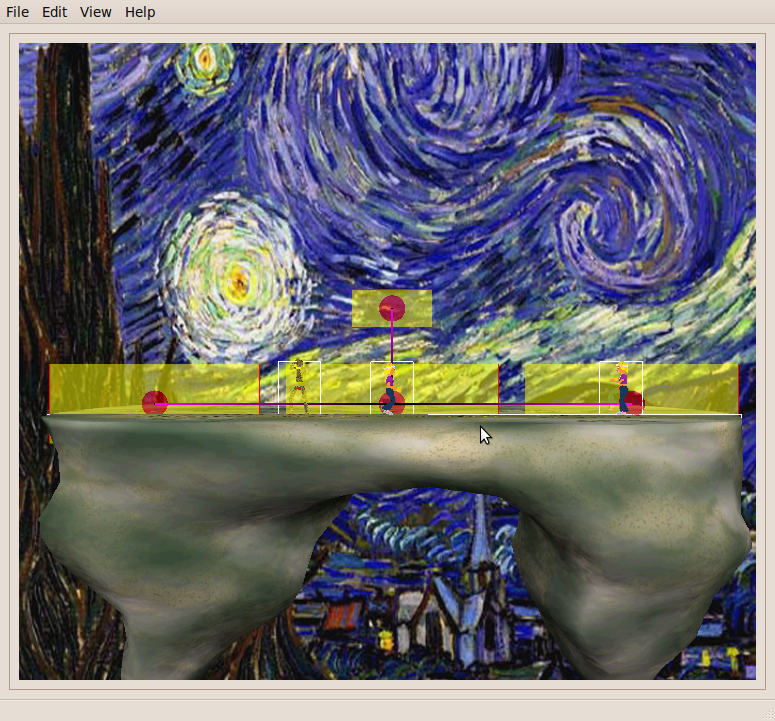
\includegraphics[scale=0.4]{visuel/capture-deplacement.png}
\caption{Graphe de déplacement : les disques rouges correspondent aux noeuds}
\end{figure}



\subsection{Déplacement d'un noeud à un autre}
\vspace{0.5cm}

\paragraph{Avant de procéder à quoi que ce soit, l'IA se posera une série de question afin de savoir quelle action effectuer. Voici ci-dessous la liste des questions : }

\begin{enumerate}
	\item \textbf{Dans quel noeud je suis ?}
	\item \textbf{Dans quel noeud se trouve mon objectif ?}\\
$\rightarrow$ On cherche à la fois où le bot se trouve dans l’arène (noeud A) et où l'objectif du bot se trouve dans l’arène (noeud B) : parcours du graphe.\\

Algorithme par position des noeuds
\begin{footnotesize}
\setlength{\itemsep}{20pt}
\begin{verbatim}
debut parcours
  * initialise un noeud temporaire bot //(position infinie)
  * initialise un deuxième noeud temporaire target //(position infinie)
  * pour chaque noeud
    * calcul de la distance (positionObjectif, positionNoeud) ;
    * la distance est-elle plus petite que celle du noeud temporaire bot ?
      - si oui : stockage du noeud dans noeud temporaire bot et continue
      - si non : continue
    * calcul de la distance (positionCible, positionNoeud) ;
    * la distance est-elle plus petite que celle du noeud temporaire target ?
      - si oui : 
        * le noeud est-il une zone dangereuse (un trou par exemple) ?
        // Ici le caracère de l'IA peut modifier les probabilités
        // afin de définir qu'est ce qui est dangereux ou qui ne l'est pas
          si oui : continue
          si non : stockage du noeud dans noeud temporaire target
      - si non : continue
  fin pour
fin parcours
\end{verbatim}
\end{footnotesize}

	\item \textbf{Comment me rendre de A à B ?}\\
$\rightarrow$ Recherche du plus court chemin dans le graphe avec l'algorithme de Dijkstra en renvoyant une liste de noeuds
\\\\
\textbf{a) Hypothèse 1}\\
Dans ce cas, l'action "goTo" reste en tête de file tant qu'elle n'est pas accomplie.\\
Problème : risque de croiser le joueur vers lequel il se dirigeait et de l'ignorer jusqu'à avoir atteint l'ancienne position.\\
Solution : des intervalles entre les zones clés pas trop éloignés.\\
\\
\textbf{b) Hypothèse 2} (redéfinition de B)\\
L'action "goTo" est mise à jour à chaque rafra\^ichissement de radar mais pas défilé (seules les coordonnées d'arrivée changent). Elle est défilée seulement lorsque les coordonnées d'arrivée sont atteintes.\\
\textbf{Problème} : lorsque l'objectif est d'éviter la cible / joueur, il faut définir une cible (zone-clé) qui soit la plus éloignée possible de lui. Cela revient à faire un parcours en profondeur en plus pour touver le noeud le plus éloigné.\\
\textbf{Solution} : l'implémentation d'une action "flee" différenciée de "goTo" qui parcours le graphe non pas pour trouver le chemin le plus court entre A et B mais pour trouver le chemin le plus long en partant de B et passant par A (sans jamais repasser par le même noeud). Puis de retourner seulement le chemin à partir de A.
\\\\
\textbf{c) Hypothèse 3} (B non ponctuel)\\
L'action "goTo" n'est pas implémentée telle quelle mais plutôt par des rayons d'action centrés sur la cible qui agiraient comme suit : fuir (rayon maximal), se rapprocher (rayon minimal, ou en tout cas à portée d'attaque), se rapprocher pour tirer (rayon égal à la portée d'un projectile), se maintenir à une certaines distance de la cible (un certain rayon). L'action "goTo" dispara\^it alors de la file comme les autres, quand l'objectif est atteint.\\
\textbf{Problème} : que faire si le bot ne peut pas atteindre le cercle (si le joueur tombe et que le bot doit l'attaquer par exemple) ?\\
\textbf{Solution 1} : le demi cercle subit constamment des variations de rayon aléatoires obligeant le bot à se remettre en mouvement. \\
\textbf{Solution 2} (ou complémentaire) : lorsque le bot est resté inactif (obligation d'implémenter une action "attente") un certain nombre de frame dépendant de son caractère, il change de stratégie (attaque à distance par exemple). 
 
\end{enumerate}
 


\subsection{Amélioration de l'IA}

\paragraph{Le fait de n'effectuer qu'une seule action puis une autre puis une autre sans lien entre ces dernières ne semble pas très "réaliste". Lorsqu'on joue à un jeu de baston, les meilleurs sont ceux qui établissent des stratégies (même si celles-ci se résument à appuyer sur tous les boutons frénétiquement dans l'espoir de toucher son adversaire). Un stratégie signifie des actions qui ont un lien entre elles. Ce choix est justifié par le nombre des actions à disposition : un bot pourra n'attaquer qu'à distance pendant un certain temps pour affaiblir son adversaire tout en se tenant éloigné de ses coups puis passer à l'attaque au corps à corps, mais un autre pourra au contraire décider de privilégier une série d'attaques au corps à corps. Dans les deux cas, on se rend compte qu'un simple random sur les actions du bot ne suffit pas à simuler une intelligence. La solution proposée est simple : \textbf{plutôt que de choisir au hasard avec des probabilités homogènes la prochaine action à effectuer, les probabilités sont affectées}. Prenons un exemple : }

\paragraph{Soit Bob un bot au caratère plutôt défensif. Bob se fait attaquer par un joueur plutôt belliqueux.
Bob se protège d'un coup. Quelle est sa prochaine action ? Il peut : }
\begin{itemize}
	\item Fuir à droite (20\%)
	\item Fuir à gauche (20\%)
	\item Attaquer (20\%)
	\item Lancer un projectile (20\%)
	\item Continuer à se protéger (20\%)
\end{itemize}

\paragraph{Pour le moment, toutes les actions ont 20\% de chance de se réaliser mais à l'évidence certaine de ces propositions subiront un malus à leur probabilité. Bob est défensif, la probabilité qu'il attaque ou qu'il lance un projectile est faible et est donc divisée par deux (passant à 10\%) tandis que la probabilité qu'il se protège ou tente de fuir augmente. Bob s'est protégé à l'action précédente, si la situation n'a pas changé et que le joueur belliqueux est toujours à portée, le choix pour l'action précédente est toujours valide, la probabilité de "se protéger" reçoit donc un nouveau bonus. Le tirage aléaoire se fera donc avec les probabilités suivantes :}

\begin{itemize}
	\item Fuir à droite (25\%)
	\item Fuir à gauche (25\%)
	\item Attaquer (10\%)
	\item Lancer un projectile (10\%)
	\item Continuer à se protéger (30\%)
\end{itemize}


\paragraph{On se rend compte qu'en réalité deux passes ont été faites : la première modifie les probabilités en fonction du caractère, la seconde en fonction de la situation (a-t-elle évoluée de manière radicale?).}

\paragraph{Bien sûr, cette methode diffère peu de la première mais le bot semble posséder tout de même une once d'intelligence. Si l'on veut poursuivre dans cette voie, il est facile de multiplier les facteurs intervenant sur les probabilités pour affiner le choix final et le rendre d'une certaine façon plus cohérent. Il serait bon pour éviter à une action de se répéter excessivement de fixer un pallier de probabilité à 50\%.}

\paragraph{Revenons à la barette d'action de la classe "Brain". Pourquoi avoir une barette d'actions ?\\
Ce tableau organisé comme une pile dans un premier temps, puis comme une file dans un second, contient un nombre prédéfini d'actions qui aiderons / orienterons le choix de l'IA de manière plus précise.}

\begin{footnotesize}
\begin{verbatim}
// on a rempli la liste au démarrage de manière aléatoire
// (parmi les actions liées au caractère du bot)
* à chaque fois que l'IA reçoit le radar
  * initialise une liste de taille x
  * détruit le plus ancien maillon
  * pour tous les éléments de la barette d'action
    * modification des probabilités en conséquence
  fin pour
  // Prise effective de la décision
  * ajoute l'action issu de la décision dans la nouvelle liste
  * la nouvelle liste prend la place de l'ancienne
fin chaque
\end{verbatim}
\end{footnotesize}

\paragraph{La methode qui aurait été implémentée si nous avions eu le temps parait la plus aboutie des trois (même s'il est difficile de l'évaluer correctement sans l'avoir observée en pratique) est la suivante : l'\textbf{implémentation d'une mémoire}.}

\paragraph{En effet là où nous, joueur, pouvons observer les tendances des adversaires, l'IA ne peut rien. Nous avons donc décider de la doter d'une mémoire afin de rajouter un maillon essentiel au processus de décision qui est : l'évaluation des conséquences de ses choix précédents. Le principe est simple : si un chien fait une bêtise il sera grondé, il saura qu'il a fait une erreur et ne recommencera pas, au contraire si on lui donne un sucre suite à son double salto arrière, alors il le fera plus souvent et en épatera plus d'un ! Notre IA doit donc être capable de se souvenir si tel ou tel de ses actions ont eu de bonnes répercussions ou non (dans notre jeu et pour simplifier, si le bot a fait des dégâts ou bien en a encaissé).}

\paragraph{L'implémentation est réalisée comme suit : l'IA possède deux arbres formés de toutes les combinaisons possibles, un pour l'attaque, un pour la défense. La taille des arbres est liée au nombre d'actions disponibles et à la capacité de sa mémoire, dans notre cas et avec des enchainements qui ne dépassent pas plus de cinq actions, la complexité reste raisonnable. Chaque fois que l'IA est sollicitée, elle fait le bilan de son précédent encha\^inement et incrémente en fonction les probabilités dans l'arbre. Certains encha\^inements se verront donc privilégiés par rapport à d'autres (note: pour augmenter la difficulté d'une IA, augmenter la taille des encha\^inements permet une mesure plus précise et un choix d'autant plus adapté à la situation). Il est bien sûr possible en poursuivant le raisonnement de stocker ces arbres dans des fichiers si l'IA est amené à rencontrer plusieurs fois le même adversaire afin qu'elle "apprenne" son style de jeu (nécessite l'implémentation de profils de joueurs).}



\newpage
\section{Gestion du son}
\subsection{Mise en place du son}
\paragraph{Il nous a semblé inconcevable de faire un jeu sans son, l’ambiance sonore étant presque aussi important que l’image pour l’immersion dans le jeu.}

\paragraph{Nous avons donc fait le choix d’une bibliothèque pour le son. Il en existe plusieurs, notamment \textit{SDL\_mixer} et \textit{fmod}, les deux étant aussi performantes, de complexité d’utilisation similaire. N’utilisant pas déjà \textit{SDL}, nous avons choisi arbitrairement \textit{fmod}.}

\paragraph{Après quelques difficultés d’installation, la bibliothèque était opérationnelle, fonctionnant sous GNU/Linux 32 ou 64 bits.}

\paragraph{Nous avons créé une classe \textbf{Sound} adaptée pour le jeu, utilisant certaines fonctions de \textit{fmod}, afin de pouvoir jouer des sons aux moments appropriés dans le jeu de façon simple et pratique.}

\paragraph{Cette classe permet les actions suivantes :}
\begin{itemize}
	\item Initialisation et création d’un système sonore qui sera utilisé pour tous les sons (méthode statique). En cas d’échec, le jeu ne dois pas être perturbé donc la classe est conçue pour continuer à fonctionner mais sans son
	\item Chargement d’une musique depuis un fichier, qui sera jouée en streaming pour ne pas surcharger la mémoire
	\item Chargement d’un petit son depuis un fichier, qui sera lu dans la mémoire pour pouvoir être lu rapidement (correspond aux voix et effets qui sont joués à plusieurs reprises durant le jeu).
	\item Au chargement, on précise si le son sera joué en boucle ou non
	\item Lecture / Arrêt d’un son
	\item Ajout d’un effet (écho, flanger, lowpass, highpass, etjenpass…)
	\item Ajustage du volume d’un son seul
	\item Ajustage du volume de tous les sons de type « musique »
	\item Ajustage du volume de tous les sons de type « effets/voix »
	\item Ajustage du volume général
\end{itemize}

\paragraph{Nous avons mis en place un réglage du volume général, des effets et de la musique via une fenêtre « préférences » accessible depuis le menu QT.}


\subsection{Choix des sons}
\paragraph{Nous avons choisi de lancer une musique globale qui se répète en boucle tout le long du jeu. Cette musique vient du jeu vidéo \textit{Super Smash Bros Brawl} et correspond bien à l’ambiance souhaitée, en particulier pour l’arène « Rome » actuellement utilisée.
Ensuite, pour chaque personnage, nous utilisons des bruitages ou voix qui sont joués lors de certains événements, par exemple, donner un coup ou s'en prendre un. Des sons seront aussi choisis pour être ajoutés aux effets spéciaux, par exemple lors de certaines attaques, victoire, etc.\\
Nous envisageons aussi d’utiliser des effets sonores sur les sons ou la musique lors de certains événements.}



\subsection{Améliorations possibles}
\paragraph{Il aurait été bien d’approfondir la gestion sonore, en ajoutant des effets plus évolués à certains moments, en utilisant plus de sons différents, en créant des sons nous-mêmes pour certaines voix par exemple.}
\paragraph{Des sons pourraient aussi être joués à d’autres moments que ce qui a été fait.}
\paragraph{Il serait par ailleurs intéressant de mettre plus de musiques, différentes selon les arènes, et différentes selon qu’on joue, qu’on est en pause ou qu’on est sur un menu.}
\paragraph{Enfin des bruitages pourraient être ajoutés comme ambiance pour les arènes (pluie, vent, oiseaux, applaudissements) pour une meilleure immersion.}

\newpage
\section{Principe du jeu}

 
 
\subsection{Guide utilisateur}

\paragraph{\textbf{Rappel du principe du jeu} : }
\paragraph{Smashtein Garbage est un jeu qui s'inspire fortement du célébre jeu \textit{Super Smash Bros Brawl}.}
\paragraph{Le but du jeu consiste à se taper dessus jusqu'à éjecter un joueur de l'arène ou jusqu'à épuisement de ses points de vie. Chaque robot possède un certain nombre de vies. Lorsqu'il n'y a plus de vie, le robot est éliminé. Le vainqueur sera donc le dernier restant.}

\vspace{0.5cm}

\paragraph{Au démarrage du jeu, un écran d'introduction appara\^it permettant de présenter le logo de notre jeu. L'écran suivant affiche le choix de l'avatar ainsi que de l'arène. Attention, que le combat commence !}

\paragraph{Contr\^olez votre avatar avec les touches directionnelles de votre clavier. Via la barre de menu, il est possible de changer de vue. Des raccourcis claviers y sont associés :}

\begin{itemize}
	\item[$\triangleright$ Caméra poursuite] (\verb?CTRL+F1?) : suit un personnage
	\item[$\triangleright$ Vue globale] (\verb?CTRL+F2?) : vue d'ensemble de tous les personnages
	\item[$\triangleright$ Caméra debug] (\verb?CTRL+F3?) : permet de parcourir l'environnement en mode sphérique
	\item[$\triangleright$ Caméra libre] (\verb?CTRL+F4?) : permet de parcourir l'environnement en vue FPS\footnote{First Person Shooter}
	\item[$\triangleright$ Mode multi-vue] (\verb?CTRL+F5?) : affiche les 4 vues précédentes simultanément
\end{itemize}

\vspace{0.5cm}

\paragraph{Il est possible de \textbf{régler le niveau du son général}, de la \textbf{musique} et des \textbf{effets sonores} via le panneau de préférences. Ces préférences sont accessibles depuis la barre de menu ou depuis le raccourci \verb?CTRL+P?}


\newpage
\chapter*{4. Conclusion}
\addcontentsline{toc}{chapter}{4. Conclusion}
\paragraph{Pour conclure, la réalisation du projet Smashstein s’est révélée comme une expérience très instructive et enrichissante en tout point.}

\paragraph{Premièrement, elle nous aura permis de réaliser un véritable jeu vidéo dans des conditions proches de celles du travail en entreprise puisqu’au sein de la relativement grande équipe de ce projet, chacun a pu réellement se spécialiser afin de valoriser au mieux ses compétences propres et travailler de manière d’autant plus efficace.}

\paragraph{Par ailleurs ce projet a été l’occasion d’approfondir nos connaissances et de nous aguerrir dans divers domaines. Bien entendu, la programmation C++ a joué un rôle central et nous avons pu grandement pratiquer ce langage en découvrant au passage de nouvelles bibliothèques. L’utilisation des logiciels de modélisation \textit{3D} que sont \textit{Blender} et \textit{3DS MAX} a également été cruciale. Cependant, l’aspect le plus intéressant reste la découverte des mécanismes de combinaison de ces domaines qui n’avaient été abordés en cours que séparément jusqu’à présent.}

\paragraph{Enfin, s’il fallait émettre un avis sur notre travail, nous pourrions dire que, même si le résultat est encore perfectible sur certains points, \textit{Smashtein Garbage} remplit toutes les fonctionnalités demandées de manière satisfaisante et en apporte même de nouvelles. Nous sommes donc plutôt satisfaits du résultat, même si nous aurions aimé passer plus de temps sur la partie esthétique du jeu afin d’aboutir sur des décors et personnages plus jolis, mais aussi pourquoi pas de composer nos propres sons et mélodies à l’aide d’un logiciel comme \textit{Rosegarden}.}

\newpage
\renewcommand\bibname{5. Bibliographie}


\begin{thebibliography}{99}
	\bibitem _Documentation officielle QT 4.0 [en] : \url{http://doc.trolltech.com/4.0/}
	\bibitem _J. \textsc{Siek}, L. \textsc{Lee}, A. \textsc{Lumsdaine}, The Boost Graph Library, User Guide and Reference Manual, Addison-Wesley, 2002 	
	\bibitem _FAQ LaTeX [en] : \url{http://www.tex.ac.uk/cgi-bin/texfaq2html?introduction=yes}	
	\bibitem _Aide LaTeX [fr] : \url{http://latex.developpez.com/faq/}
\end{thebibliography}
\addcontentsline{toc}{chapter}{5. Bibliographie}


%%%%%%%%%%%%%%%%%%%%%%%%%%%%%%%%% Annexe %%%%%%%%%%%%%%%%%%%%%%%%%%%%%%%%%
\newpage
\appendix
\chapter*{6. Annexes}
\addcontentsline{toc}{chapter}{6. Annexes}
\setcounter{chapter}{1}
\section{Quelques captures d'écran}
\begin{figure}[h]
	\center
	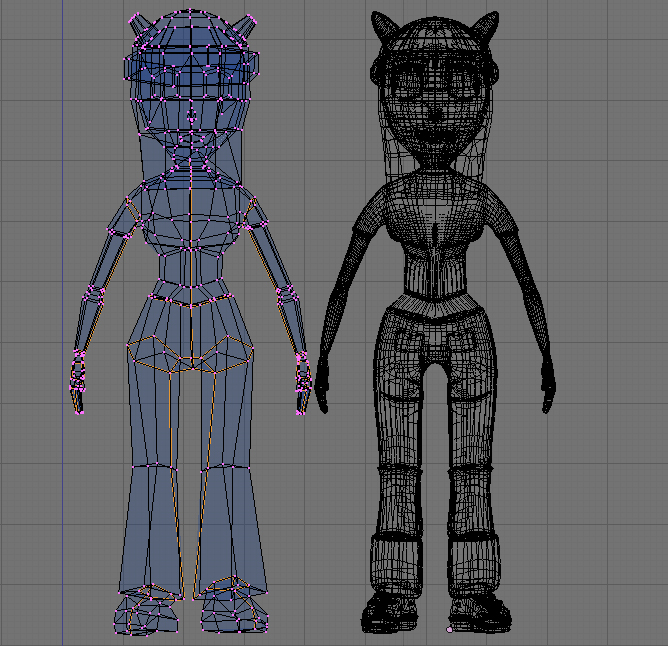
\includegraphics[scale=0.4]{visuel/mesh.jpg}
	\caption{Visualisation des meshes}
\end{figure}

\begin{figure}[!h]
	\center
	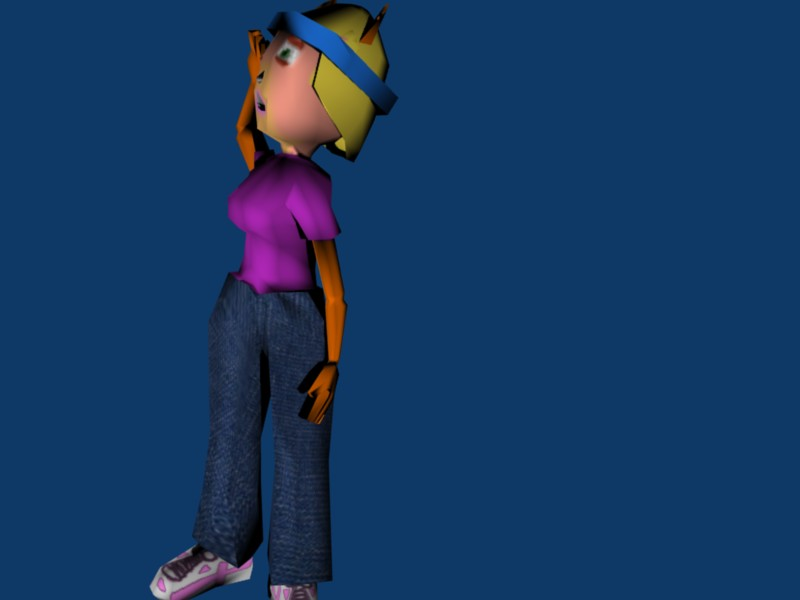
\includegraphics[scale=0.4]{visuel/rendu_test1.jpg}
	\caption{Test de rendu d'un personnage}
\end{figure}

\begin{figure}[!h]
	\center
	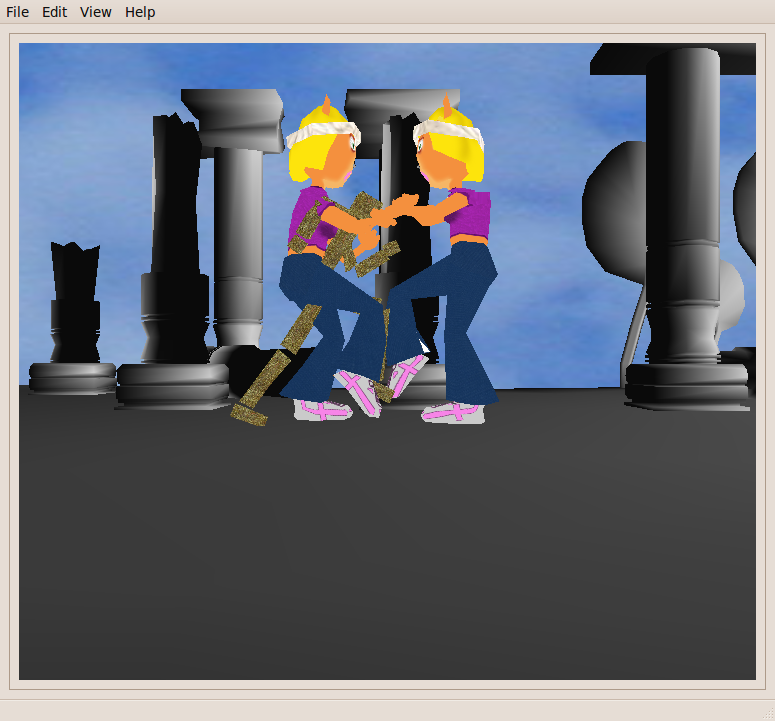
\includegraphics[scale=0.4]{visuel/capture-rev140-1.png}
	\caption{Vue globale de l'arène}
\end{figure}

\newpage
\section{Pseudo-code de l'IA}

\begin{scriptsize}
\begin{verbatim}
Toutes les x frames : regarde s'il change de comportement (modulé par le comportement)


actions possibles :

direction droite
direction gauche
sauter
coup1
coup2
projectile
bloquer

_______________________________________________________________

structures de données :

arbre attaque
arbre defense
barette mémoire (file) "enchainement player" (même nb de barettes que de joueur)  
barette mémoire (file) "enchainement bot"
barette action (file)

recupération d'un argument de main pour le profil du joueur
stockage des arbres de probabilités dans les fichiers textes

_______________________________________________________________

RECUPERATION DU RADAR + ACCES A LA MEMOIRE

qui est mon ennemi ?
  * y a-t-il plus d'un ennemi ?
    -> si non : 
      * le choix est fait
    -> si oui : 
      * choix entre différentes propositions
      -> quel est mon caractère ? (agressif, peureux, vengeur, etc...)
      /*
      Critères de selection
      si ennemi est très très bas en PV alors l'option correspondante recevra un bonus enorme
      si un ennemi a infligé + de 50 % de dégâts (pourcentage modulé par le caractère) alors il cherche a se venger
      si un ennemi a reçu + de 50 % de dégâts (idem) alors il va chercher à l'achever
      si les probabilités sont proches entre elles alors l'option "plus près" 
      */
	
        -> le plus près
        -> le plus mal en point
        -> celui qui a infligé le plus de dégât
        -> celui qui a été le plus tapé

remplit la mémoire sur l'action précédente
  * quelle a été l'action du player ?
    * si la barette contient X (un seuil pédéfini) actions alors reset de la barette
    * si la dernière entrée de la barette date d'au moins X frame alors reset de la barette
    * enregistrement de l'action dans une barette mémoire temporaire "enchainement player"
  * le bot a-t-il fait des dommages ?
    -> si non : 
      * si la barette contient X (un seuil pédéfini) actions alors reset de la barette
      * si la dernière entrée de la barette date d'au moins X frame alors reset de la barette 
      * enregistrement de l'action précédente dans une barette mémoire temporaire "enchainement bot"
    -> si oui :
      * mise à jour du graphe d'attaque en parcourant selon l'enchainement effectué
  * le bot a-t-il encaisser des dommages ?
    -> si oui :
      * récupération de la barette temporaire "enchainement player"
      * mise à jour du graphe de defense en parcourant selon l'enchainement effectué (malus)
    -> si non :
      * récupération de la barette temporaire "enchainement player"
      * la dernière entrée de la barette date de moins X frame (obsolète)
        -> si oui : 
          * reset de la barette
        -> si non :
          * mise à jour du graphe de defense en parcourant selon l'enchainement effectué (bonus)   
			
quel est mon état ? choix :
  -> quel est mon caractère ? (agressif, peureux, vengeur, etc...)
	
  /*
  Notes comportement
  Certains possèdent des conditions ("instructions prioritaires")
  Exemple : agressif ne doit pas laisser de repos à son adversaire 
  (pas attendre avant d'attaquer) et doit se trouver à middle range de sa cible
  */
	
    -> attaque
    -> défense
		
ai-je suffisamment de probabilités pour cet ennemi ? 
// seuil fixé dans les arbres de proba et modulé par le caractère
  -> si non : 
    * comportement passe à "recherche information"
    // c'est-à-dire remplir l'arbre de probabilité correspondant)
		
    /*
    Notes "recherche information"
    Parcours de l'arbre correspondant.
    Si une inconnue est rencontré sa priorité devient maximale,
    si plusieurs inconnues existent alors choix aleatoire. 
    */
		
    -> si oui : 
      * alors parcours de l'arbre de probabilité correspondant
        -> comportement X

mise à jour de la barette d'action
  * remplir la barette avec les actions données par la comportement
    -> y a-t-il un événement majeur ?
    // apparition super bonus, point de vie proche de zéro, se maintenir à middle range
      -> si oui :
        * insérer cette action en tête de barette stratégie
			
  * vérifié la validité de l'action (si elle n'a pas déjà été faite)		
  * lancer la première action de la barette
\end{verbatim}
\end{scriptsize}



\end{document}